% Options for packages loaded elsewhere
\PassOptionsToPackage{unicode}{hyperref}
\PassOptionsToPackage{hyphens}{url}
%
\documentclass[
]{article}
\usepackage{amsmath,amssymb}
\usepackage{iftex}
\ifPDFTeX
  \usepackage[T1]{fontenc}
  \usepackage[utf8]{inputenc}
  \usepackage{textcomp} % provide euro and other symbols
\else % if luatex or xetex
  \usepackage{unicode-math} % this also loads fontspec
  \defaultfontfeatures{Scale=MatchLowercase}
  \defaultfontfeatures[\rmfamily]{Ligatures=TeX,Scale=1}
\fi
\usepackage{lmodern}
\ifPDFTeX\else
  % xetex/luatex font selection
\fi
% Use upquote if available, for straight quotes in verbatim environments
\IfFileExists{upquote.sty}{\usepackage{upquote}}{}
\IfFileExists{microtype.sty}{% use microtype if available
  \usepackage[]{microtype}
  \UseMicrotypeSet[protrusion]{basicmath} % disable protrusion for tt fonts
}{}
\makeatletter
\@ifundefined{KOMAClassName}{% if non-KOMA class
  \IfFileExists{parskip.sty}{%
    \usepackage{parskip}
  }{% else
    \setlength{\parindent}{0pt}
    \setlength{\parskip}{6pt plus 2pt minus 1pt}}
}{% if KOMA class
  \KOMAoptions{parskip=half}}
\makeatother
\usepackage{xcolor}
\usepackage[margin=1in]{geometry}
\usepackage{color}
\usepackage{fancyvrb}
\newcommand{\VerbBar}{|}
\newcommand{\VERB}{\Verb[commandchars=\\\{\}]}
\DefineVerbatimEnvironment{Highlighting}{Verbatim}{commandchars=\\\{\}}
% Add ',fontsize=\small' for more characters per line
\usepackage{framed}
\definecolor{shadecolor}{RGB}{248,248,248}
\newenvironment{Shaded}{\begin{snugshade}}{\end{snugshade}}
\newcommand{\AlertTok}[1]{\textcolor[rgb]{0.94,0.16,0.16}{#1}}
\newcommand{\AnnotationTok}[1]{\textcolor[rgb]{0.56,0.35,0.01}{\textbf{\textit{#1}}}}
\newcommand{\AttributeTok}[1]{\textcolor[rgb]{0.13,0.29,0.53}{#1}}
\newcommand{\BaseNTok}[1]{\textcolor[rgb]{0.00,0.00,0.81}{#1}}
\newcommand{\BuiltInTok}[1]{#1}
\newcommand{\CharTok}[1]{\textcolor[rgb]{0.31,0.60,0.02}{#1}}
\newcommand{\CommentTok}[1]{\textcolor[rgb]{0.56,0.35,0.01}{\textit{#1}}}
\newcommand{\CommentVarTok}[1]{\textcolor[rgb]{0.56,0.35,0.01}{\textbf{\textit{#1}}}}
\newcommand{\ConstantTok}[1]{\textcolor[rgb]{0.56,0.35,0.01}{#1}}
\newcommand{\ControlFlowTok}[1]{\textcolor[rgb]{0.13,0.29,0.53}{\textbf{#1}}}
\newcommand{\DataTypeTok}[1]{\textcolor[rgb]{0.13,0.29,0.53}{#1}}
\newcommand{\DecValTok}[1]{\textcolor[rgb]{0.00,0.00,0.81}{#1}}
\newcommand{\DocumentationTok}[1]{\textcolor[rgb]{0.56,0.35,0.01}{\textbf{\textit{#1}}}}
\newcommand{\ErrorTok}[1]{\textcolor[rgb]{0.64,0.00,0.00}{\textbf{#1}}}
\newcommand{\ExtensionTok}[1]{#1}
\newcommand{\FloatTok}[1]{\textcolor[rgb]{0.00,0.00,0.81}{#1}}
\newcommand{\FunctionTok}[1]{\textcolor[rgb]{0.13,0.29,0.53}{\textbf{#1}}}
\newcommand{\ImportTok}[1]{#1}
\newcommand{\InformationTok}[1]{\textcolor[rgb]{0.56,0.35,0.01}{\textbf{\textit{#1}}}}
\newcommand{\KeywordTok}[1]{\textcolor[rgb]{0.13,0.29,0.53}{\textbf{#1}}}
\newcommand{\NormalTok}[1]{#1}
\newcommand{\OperatorTok}[1]{\textcolor[rgb]{0.81,0.36,0.00}{\textbf{#1}}}
\newcommand{\OtherTok}[1]{\textcolor[rgb]{0.56,0.35,0.01}{#1}}
\newcommand{\PreprocessorTok}[1]{\textcolor[rgb]{0.56,0.35,0.01}{\textit{#1}}}
\newcommand{\RegionMarkerTok}[1]{#1}
\newcommand{\SpecialCharTok}[1]{\textcolor[rgb]{0.81,0.36,0.00}{\textbf{#1}}}
\newcommand{\SpecialStringTok}[1]{\textcolor[rgb]{0.31,0.60,0.02}{#1}}
\newcommand{\StringTok}[1]{\textcolor[rgb]{0.31,0.60,0.02}{#1}}
\newcommand{\VariableTok}[1]{\textcolor[rgb]{0.00,0.00,0.00}{#1}}
\newcommand{\VerbatimStringTok}[1]{\textcolor[rgb]{0.31,0.60,0.02}{#1}}
\newcommand{\WarningTok}[1]{\textcolor[rgb]{0.56,0.35,0.01}{\textbf{\textit{#1}}}}
\usepackage{graphicx}
\makeatletter
\def\maxwidth{\ifdim\Gin@nat@width>\linewidth\linewidth\else\Gin@nat@width\fi}
\def\maxheight{\ifdim\Gin@nat@height>\textheight\textheight\else\Gin@nat@height\fi}
\makeatother
% Scale images if necessary, so that they will not overflow the page
% margins by default, and it is still possible to overwrite the defaults
% using explicit options in \includegraphics[width, height, ...]{}
\setkeys{Gin}{width=\maxwidth,height=\maxheight,keepaspectratio}
% Set default figure placement to htbp
\makeatletter
\def\fps@figure{htbp}
\makeatother
\setlength{\emergencystretch}{3em} % prevent overfull lines
\providecommand{\tightlist}{%
  \setlength{\itemsep}{0pt}\setlength{\parskip}{0pt}}
\setcounter{secnumdepth}{-\maxdimen} % remove section numbering
\ifLuaTeX
  \usepackage{selnolig}  % disable illegal ligatures
\fi
\IfFileExists{bookmark.sty}{\usepackage{bookmark}}{\usepackage{hyperref}}
\IfFileExists{xurl.sty}{\usepackage{xurl}}{} % add URL line breaks if available
\urlstyle{same}
\hypersetup{
  pdftitle={bacs\_hw4},
  pdfauthor={110071010},
  hidelinks,
  pdfcreator={LaTeX via pandoc}}

\title{bacs\_hw4}
\author{110071010}
\date{2024-03-14}

\begin{document}
\maketitle

\textbf{110070011} has helped me find the slider bars of
interactive\_t\_test(). Originally I didn't run the code in the console,
so they didn't show up.

\hypertarget{question-1}{%
\section{Question 1}\label{question-1}}

The large American phone company Verizon had a monopoly on phone
services in many areas of the US. The New York Public Utilities
Commission (PUC) regularly monitors repair times with customers in New
York to verify the quality of Verizon's services. The file verizon.csv
has a recent sample of repair times collected by the PUC.

\hypertarget{a}{%
\subsection{1a}\label{a}}

\hypertarget{instruction}{%
\subsubsection{Instruction}\label{instruction}}

Imagine that Verizon claims that they take 7.6 minutes to repair phone
services for its customers on average. The PUC seeks to verify this
claim at 99\% confidence (i.e., significance alpha = 1\%) using
traditional statistical methods.

\hypertarget{my-solution}{%
\subsubsection{My Solution}\label{my-solution}}

\hypertarget{i-visualize-the-distribution-of-verizons-repair-times-marking-the-mean-with-a-vertical-line}{%
\paragraph{(i) Visualize the distribution of Verizon's repair times,
marking the mean with a vertical
line}\label{i-visualize-the-distribution-of-verizons-repair-times-marking-the-mean-with-a-vertical-line}}

\begin{Shaded}
\begin{Highlighting}[]
\CommentTok{\# Read in the dataset}
\NormalTok{data }\OtherTok{\textless{}{-}} \FunctionTok{read.csv}\NormalTok{(}\StringTok{"verizon.csv"}\NormalTok{)}
\NormalTok{sample\_vrt }\OtherTok{\textless{}{-}}\NormalTok{ data}\SpecialCharTok{$}\NormalTok{Time}

\CommentTok{\# Get a glimpse into the distribution }
\FunctionTok{plot}\NormalTok{(}\FunctionTok{density}\NormalTok{(sample\_vrt),}\AttributeTok{lwd =}\DecValTok{2}\NormalTok{, }\AttributeTok{col =} \StringTok{"blue"}\NormalTok{, }\AttributeTok{main =} \StringTok{"Distribution of Verision Repair Times"}\NormalTok{)}
\FunctionTok{abline}\NormalTok{(}\AttributeTok{v =} \FunctionTok{mean}\NormalTok{(sample\_vrt))}
\end{Highlighting}
\end{Shaded}

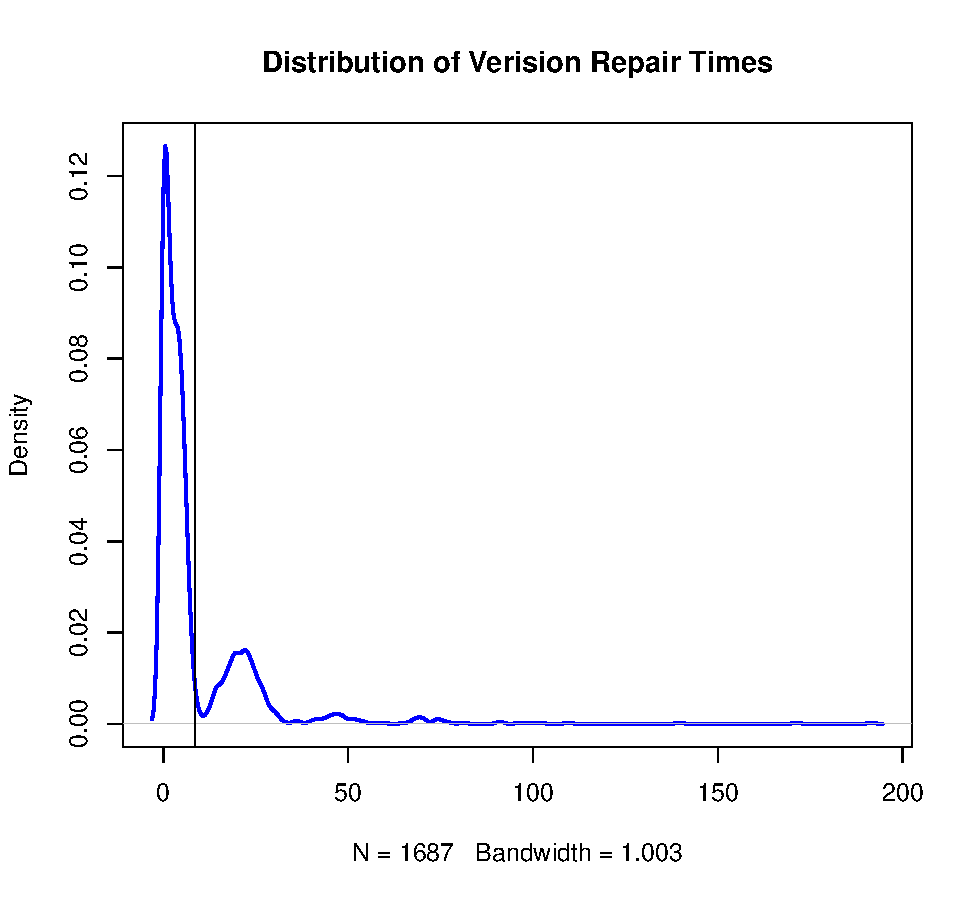
\includegraphics{bacs_hw4_files/figure-latex/unnamed-chunk-1-1.pdf}

\hypertarget{ii-given-what-the-puc-wishes-to-test-how-would-you-write-the-hypothesis}{%
\paragraph{(ii) Given what the PUC wishes to test, how would you write
the
hypothesis?}\label{ii-given-what-the-puc-wishes-to-test-how-would-you-write-the-hypothesis}}

\textbf{Null Hypothesis H0} : Population mean is equal to 7.6 mins\\
\textbf{Alternative Hypothesis H1} : Population mean is not equal to 7.6
mins

\hypertarget{iii-estimate-the-population-mean-and-the-99-confidence-interval-ci-of-this-estimate.}{%
\paragraph{(iii) Estimate the population mean, and the 99\% confidence
interval (CI) of this
estimate.}\label{iii-estimate-the-population-mean-and-the-99-confidence-interval-ci-of-this-estimate.}}

\begin{Shaded}
\begin{Highlighting}[]
\NormalTok{vrt\_size }\OtherTok{\textless{}{-}} \FunctionTok{length}\NormalTok{(sample\_vrt)}
\NormalTok{vrt\_mean }\OtherTok{\textless{}{-}} \FunctionTok{mean}\NormalTok{(sample\_vrt)}
\NormalTok{vrt\_sd }\OtherTok{\textless{}{-}} \FunctionTok{sd}\NormalTok{(sample\_vrt)}
\NormalTok{vrt\_se }\OtherTok{\textless{}{-}}\NormalTok{ vrt\_sd}\SpecialCharTok{/}\FunctionTok{sqrt}\NormalTok{(vrt\_size)}
\NormalTok{vrt\_ci99 }\OtherTok{\textless{}{-}}\NormalTok{ vrt\_mean }\SpecialCharTok{+} \FunctionTok{c}\NormalTok{(}\SpecialCharTok{{-}}\FloatTok{2.58}\SpecialCharTok{*}\NormalTok{vrt\_se, }\FloatTok{2.58}\SpecialCharTok{*}\NormalTok{vrt\_se) }\CommentTok{\# 99\% CI}

\FunctionTok{cat}\NormalTok{(}\StringTok{"Sample Mean:"}\NormalTok{, vrt\_mean, }\StringTok{"}\SpecialCharTok{\textbackslash{}n}\StringTok{"}\NormalTok{)}
\FunctionTok{cat}\NormalTok{(}\StringTok{"Standard Error:"}\NormalTok{, vrt\_se, }\StringTok{"}\SpecialCharTok{\textbackslash{}n}\StringTok{"}\NormalTok{)}
\FunctionTok{cat}\NormalTok{(}\StringTok{"99\% Confidence Interval:"}\NormalTok{, }
    \StringTok{"}\SpecialCharTok{\textbackslash{}n}\StringTok{"}\NormalTok{,}\StringTok{"Lower Bound ="}\NormalTok{, vrt\_ci99[}\DecValTok{1}\NormalTok{], }\StringTok{"}\SpecialCharTok{\textbackslash{}n}\StringTok{"}\NormalTok{,}
    \StringTok{"Upper Bound ="}\NormalTok{, vrt\_ci99[}\DecValTok{2}\NormalTok{], }\StringTok{"}\SpecialCharTok{\textbackslash{}n}\StringTok{"}\NormalTok{)}
\end{Highlighting}
\end{Shaded}

\begin{verbatim}
## Sample Mean: 8.522009 
## Standard Error: 0.3600527 
## 99% Confidence Interval: 
##  Lower Bound = 7.593073 
##  Upper Bound = 9.450946
\end{verbatim}

\hypertarget{iv-find-the-t-statistic-and-p-value-of-the-test}{%
\paragraph{(iv) Find the t-statistic and p-value of the
test}\label{iv-find-the-t-statistic-and-p-value-of-the-test}}

\begin{Shaded}
\begin{Highlighting}[]
\NormalTok{hyp\_mean }\OtherTok{\textless{}{-}} \FloatTok{7.6} 
\NormalTok{t }\OtherTok{\textless{}{-}}\NormalTok{ (vrt\_mean }\SpecialCharTok{{-}}\NormalTok{ hyp\_mean)}\SpecialCharTok{/}\NormalTok{vrt\_se}
\NormalTok{df }\OtherTok{\textless{}{-}}\NormalTok{ vrt\_size }\SpecialCharTok{{-}}\DecValTok{1}
\NormalTok{p }\OtherTok{\textless{}{-}} \DecValTok{1}\SpecialCharTok{{-}} \FunctionTok{pt}\NormalTok{(t,df)}

\FunctionTok{cat}\NormalTok{(}\StringTok{"t{-}statistic:"}\NormalTok{, t, }\StringTok{"}\SpecialCharTok{\textbackslash{}n}\StringTok{"}\NormalTok{)}
\FunctionTok{cat}\NormalTok{(}\StringTok{"p{-}value:"}\NormalTok{, p, }\StringTok{"}\SpecialCharTok{\textbackslash{}n}\StringTok{"}\NormalTok{)}
\end{Highlighting}
\end{Shaded}

\begin{verbatim}
## t-statistic: 2.560762 
## p-value: 0.005265342
\end{verbatim}

\hypertarget{v-briefly-describe-how-these-values-relate-to-the-null-distribution-of-t}{%
\paragraph{(v) Briefly describe how these values relate to the Null
distribution of
t}\label{v-briefly-describe-how-these-values-relate-to-the-null-distribution-of-t}}

: The null distribution of the t-statistic is a theoretical distribution
that assumes the null hypothesis is true. It is centered around 0
(indicating no difference between the sample mean and the null
hypothesis mean) and has a shape determined by the degrees of freedom.

\hypertarget{vi-what-is-your-conclusion-about-the-companys-claim-from-this-t-statistic-and-why}{%
\paragraph{(vi) What is your conclusion about the company's claim from
this t-statistic, and
why?}\label{vi-what-is-your-conclusion-about-the-companys-claim-from-this-t-statistic-and-why}}

: Given that p-value is greater than 0.005 (alpha/2) , we can accept the
company's claim (H0) that their average repair times equals 7.6.

\hypertarget{b}{%
\subsection{1b}\label{b}}

\hypertarget{instruction-1}{%
\subsubsection{Instruction}\label{instruction-1}}

Let's re-examine Verizon's claim that they take no more than 7.6 minutes
on average, but this time using bootstrapped testing:

\hypertarget{my-solution-1}{%
\subsubsection{My Solution}\label{my-solution-1}}

\hypertarget{i-bootstrapped-percentile-estimate-the-bootstrapped-99-ci-of-the-population-mean}{%
\paragraph{(i) Bootstrapped Percentile: Estimate the bootstrapped 99\%
CI of the population
mean}\label{i-bootstrapped-percentile-estimate-the-bootstrapped-99-ci-of-the-population-mean}}

\begin{Shaded}
\begin{Highlighting}[]
\CommentTok{\# Setting up function}
\NormalTok{sample\_statistic }\OtherTok{\textless{}{-}} \ControlFlowTok{function}\NormalTok{(stat\_function,sample0)\{}
\NormalTok{  resample }\OtherTok{\textless{}{-}} \FunctionTok{sample}\NormalTok{(sample0,}\FunctionTok{length}\NormalTok{(sample0),}\AttributeTok{replace =} \ConstantTok{TRUE}\NormalTok{)}
  \FunctionTok{stat\_function}\NormalTok{(resample)}
\NormalTok{\}}

\CommentTok{\# Setting seed before bootstrapping}
\FunctionTok{set.seed}\NormalTok{(}\DecValTok{123123}\NormalTok{)}

\CommentTok{\# Do bootstrapping 2000 times}
\NormalTok{num\_boot }\OtherTok{\textless{}{-}} \DecValTok{2000}
\NormalTok{boot\_sample\_means }\OtherTok{\textless{}{-}} \FunctionTok{replicate}\NormalTok{(num\_boot,}\FunctionTok{sample\_statistic}\NormalTok{(mean,sample\_vrt))}

\CommentTok{\# Print estimated 99\% CI of sampling means}
\NormalTok{ci99\_boot\_means }\OtherTok{\textless{}{-}} \FunctionTok{quantile}\NormalTok{(boot\_sample\_means, }\AttributeTok{probs =} \FunctionTok{c}\NormalTok{(}\FloatTok{0.005}\NormalTok{, }\FloatTok{0.995}\NormalTok{))}
\NormalTok{ci99\_boot\_means}
\end{Highlighting}
\end{Shaded}

\begin{verbatim}
##     0.5%    99.5% 
## 7.638925 9.441972
\end{verbatim}

\hypertarget{ii-bootstrapped-difference-of-means-what-is-the-99-ci-of-the-bootstrapped-difference-between-the-sample-mean-and-the-hypothesized-mean}{%
\paragraph{(ii) Bootstrapped Difference of Means: What is the 99\% CI of
the bootstrapped difference between the sample mean and the hypothesized
mean?}\label{ii-bootstrapped-difference-of-means-what-is-the-99-ci-of-the-bootstrapped-difference-between-the-sample-mean-and-the-hypothesized-mean}}

\begin{Shaded}
\begin{Highlighting}[]
\CommentTok{\# Setting up function}
\NormalTok{bootstrapping\_mean\_diff }\OtherTok{\textless{}{-}} \ControlFlowTok{function}\NormalTok{(sample0, hypothesized\_mean)\{}
\NormalTok{  resample }\OtherTok{\textless{}{-}} \FunctionTok{sample}\NormalTok{(sample0,}\FunctionTok{length}\NormalTok{(sample0),}\AttributeTok{replace =} \ConstantTok{TRUE}\NormalTok{)}
  \FunctionTok{return}\NormalTok{(}\FunctionTok{mean}\NormalTok{(resample) }\SpecialCharTok{{-}}\NormalTok{ hypothesized\_mean)}
\NormalTok{\}}

\CommentTok{\# Setting seed before bootstrapping}
\FunctionTok{set.seed}\NormalTok{(}\DecValTok{123123}\NormalTok{)}

\CommentTok{\# Do bootstrapping 2000 times}
\NormalTok{num\_boot }\OtherTok{\textless{}{-}} \DecValTok{2000}
\NormalTok{boot\_mean\_diffs }\OtherTok{\textless{}{-}} \FunctionTok{replicate}\NormalTok{(num\_boot,}\FunctionTok{bootstrapping\_mean\_diff}\NormalTok{(sample\_vrt,hyp\_mean))}

\CommentTok{\# Print estimated 99\% CI of mean differences}
\NormalTok{ci99\_boot\_mean\_diffs }\OtherTok{\textless{}{-}} \FunctionTok{quantile}\NormalTok{(boot\_mean\_diffs, }\AttributeTok{probs =} \FunctionTok{c}\NormalTok{(}\FloatTok{0.005}\NormalTok{, }\FloatTok{0.995}\NormalTok{))}
\NormalTok{ci99\_boot\_mean\_diffs}
\end{Highlighting}
\end{Shaded}

\begin{verbatim}
##       0.5%      99.5% 
## 0.03892528 1.84197161
\end{verbatim}

\hypertarget{iii-bootstrapped-t-statistic-what-is-the-99-ci-of-the-bootstrapped-t-statistic-of-the-sample-mean-versus-the-hypothesized-mean}{%
\paragraph{(iii) Bootstrapped t-statistic: What is the 99\% CI of the
bootstrapped t-statistic of the sample mean versus the hypothesized
mean?}\label{iii-bootstrapped-t-statistic-what-is-the-99-ci-of-the-bootstrapped-t-statistic-of-the-sample-mean-versus-the-hypothesized-mean}}

\begin{Shaded}
\begin{Highlighting}[]
\CommentTok{\# Build the function for calculating t{-}stat}
\NormalTok{bootstrapping\_t\_stat }\OtherTok{\textless{}{-}} \ControlFlowTok{function}\NormalTok{(sample0, hypothesized\_mean)\{}
\NormalTok{  resample }\OtherTok{\textless{}{-}} \FunctionTok{sample}\NormalTok{(sample0,}\FunctionTok{length}\NormalTok{(sample0),}\AttributeTok{replace =} \ConstantTok{TRUE}\NormalTok{)}
\NormalTok{  diff }\OtherTok{\textless{}{-}} \FunctionTok{mean}\NormalTok{(resample) }\SpecialCharTok{{-}}\NormalTok{ hypothesized\_mean}
\NormalTok{  se }\OtherTok{\textless{}{-}} \FunctionTok{sd}\NormalTok{(resample)}\SpecialCharTok{/}\FunctionTok{sqrt}\NormalTok{(}\FunctionTok{length}\NormalTok{(resample))}
  \FunctionTok{return}\NormalTok{(}\FunctionTok{mean}\NormalTok{(resample) }\SpecialCharTok{{-}}\NormalTok{ hypothesized\_mean)}
\NormalTok{\}}

\CommentTok{\# Setting seed before bootstrapping}
\FunctionTok{set.seed}\NormalTok{(}\DecValTok{123123}\NormalTok{)}

\CommentTok{\# Do bootstrapping 2000 times}
\NormalTok{num\_boot }\OtherTok{\textless{}{-}} \DecValTok{2000}
\NormalTok{boot\_t\_stats }\OtherTok{\textless{}{-}} \FunctionTok{replicate}\NormalTok{(num\_boot,}\FunctionTok{bootstrapping\_t\_stat}\NormalTok{(sample\_vrt,hyp\_mean))}

\CommentTok{\# Print estimated 99\% CI of t\_stats}
\NormalTok{ci99\_boot\_t\_stats }\OtherTok{\textless{}{-}} \FunctionTok{quantile}\NormalTok{(boot\_t\_stats, }\AttributeTok{probs =} \FunctionTok{c}\NormalTok{(}\FloatTok{0.005}\NormalTok{, }\FloatTok{0.995}\NormalTok{))}
\NormalTok{ci99\_boot\_t\_stats}
\end{Highlighting}
\end{Shaded}

\begin{verbatim}
##       0.5%      99.5% 
## 0.03892528 1.84197161
\end{verbatim}

\hypertarget{iv-plot-the-distribution-of-the-three-bootstraps-above-on-separate-plots-draw-vertical-lines-showing-the-lowerupper-bounds-of-their-respective-99-confidence-intervals.}{%
\paragraph{(iv) Plot the distribution of the three bootstraps above on
separate plots; draw vertical lines showing the lower/upper bounds of
their respective 99\% confidence
intervals.}\label{iv-plot-the-distribution-of-the-three-bootstraps-above-on-separate-plots-draw-vertical-lines-showing-the-lowerupper-bounds-of-their-respective-99-confidence-intervals.}}

\begin{Shaded}
\begin{Highlighting}[]
\CommentTok{\# Display three plots at once}
\FunctionTok{par}\NormalTok{(}\AttributeTok{mfrow =} \FunctionTok{c}\NormalTok{(}\DecValTok{3}\NormalTok{,}\DecValTok{1}\NormalTok{))}

\CommentTok{\# bootstrapped sampling means}
\FunctionTok{plot}\NormalTok{(}\FunctionTok{density}\NormalTok{(boot\_sample\_means),}\AttributeTok{lwd =} \DecValTok{2}\NormalTok{, }\AttributeTok{main =} \StringTok{"Bootstrapped Sample Means"}\NormalTok{,}\AttributeTok{col =} \StringTok{"blue"}\NormalTok{) }
\FunctionTok{abline}\NormalTok{(}\AttributeTok{v =} \FunctionTok{quantile}\NormalTok{(boot\_sample\_means, }\AttributeTok{probs =} \FunctionTok{c}\NormalTok{(}\FloatTok{0.005}\NormalTok{, }\FloatTok{0.995}\NormalTok{), }\AttributeTok{names =} \ConstantTok{FALSE}\NormalTok{))}
\CommentTok{\# bootstrapped mean differences}
\FunctionTok{plot}\NormalTok{(}\FunctionTok{density}\NormalTok{(boot\_mean\_diffs),}\AttributeTok{lwd =} \DecValTok{2}\NormalTok{, }\AttributeTok{main =} \StringTok{"Bootstrapped Mean Diffs"}\NormalTok{,}\AttributeTok{col =} \StringTok{"blue"}\NormalTok{)}
\FunctionTok{abline}\NormalTok{(}\AttributeTok{v =} \FunctionTok{quantile}\NormalTok{(boot\_mean\_diffs, }\AttributeTok{probs =} \FunctionTok{c}\NormalTok{(}\FloatTok{0.005}\NormalTok{, }\FloatTok{0.995}\NormalTok{), }\AttributeTok{names =} \ConstantTok{FALSE}\NormalTok{))}
\CommentTok{\# bootstrapped t{-}statistics}
\FunctionTok{plot}\NormalTok{(}\FunctionTok{density}\NormalTok{(boot\_t\_stats),}\AttributeTok{lwd =} \DecValTok{2}\NormalTok{, }\AttributeTok{main =} \StringTok{"Bootstrapped t\_stats"}\NormalTok{,}\AttributeTok{col =} \StringTok{"blue"}\NormalTok{)}
\FunctionTok{abline}\NormalTok{(}\AttributeTok{v =} \FunctionTok{quantile}\NormalTok{(boot\_t\_stats, }\AttributeTok{probs =} \FunctionTok{c}\NormalTok{(}\FloatTok{0.005}\NormalTok{, }\FloatTok{0.995}\NormalTok{), }\AttributeTok{names =} \ConstantTok{FALSE}\NormalTok{))}
\end{Highlighting}
\end{Shaded}

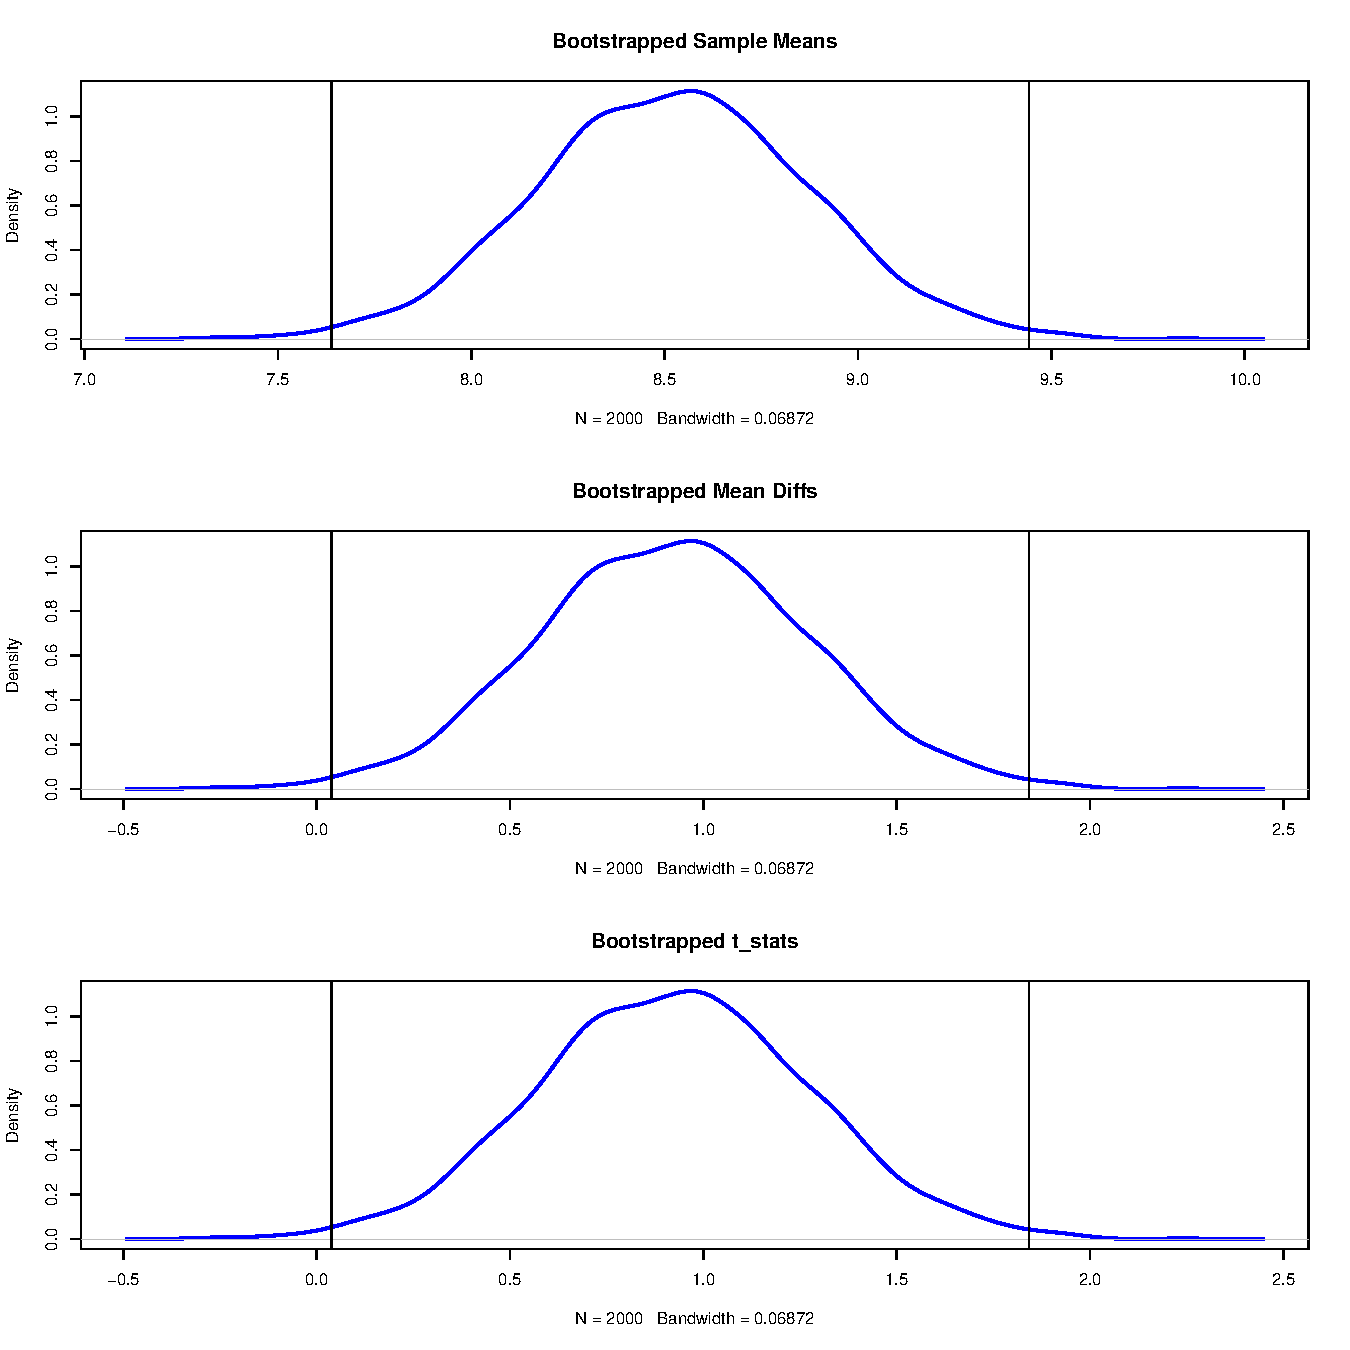
\includegraphics{bacs_hw4_files/figure-latex/unnamed-chunk-7-1.pdf}

\hypertarget{v-does-the-bootstrapped-approach-agree-with-the-traditional-t-test-in-part-a}{%
\paragraph{(v) Does the bootstrapped approach agree with the traditional
t-test in part
{[}a{]}?}\label{v-does-the-bootstrapped-approach-agree-with-the-traditional-t-test-in-part-a}}

: No, it is evident that the claimed average repair times of 7.6 mins
lies outside of the 99 \% CI of the bootstrapped statistics.

\hypertarget{c}{%
\subsection{1c}\label{c}}

\hypertarget{instruction-2}{%
\subsubsection{Instruction}\label{instruction-2}}

Finally, imagine that Verizon notes that the distribution of repair
times is highly skewed by outliers, and feel that testing the mean is
not fair because the mean is sensitive to outliers. They argue that the
median is a more fair test, and claim that the median repair time is no
more than 3.5 minutes at 99\% confidence (i.e., significance alpha =
1\%).

\hypertarget{my-solution-2}{%
\subsubsection{My Solution}\label{my-solution-2}}

\hypertarget{one-tailed-hypothesis-testing}{%
\paragraph{\texorpdfstring{\textbf{One-tailed Hypothesis
Testing}}{One-tailed Hypothesis Testing}}\label{one-tailed-hypothesis-testing}}

\textbf{Null Hypothesis H0} : population median \textless= 3.5\\
\textbf{Alternative Hypothesis} : population median \textgreater{} 3.5

\hypertarget{i-bootstrapped-percentile-estimate-the-bootstrapped-99-ci-of-the-population-median}{%
\paragraph{(i) Bootstrapped Percentile: Estimate the bootstrapped 99\%
CI of the population
median}\label{i-bootstrapped-percentile-estimate-the-bootstrapped-99-ci-of-the-population-median}}

\begin{Shaded}
\begin{Highlighting}[]
\CommentTok{\# Get the function ready}
\NormalTok{sample\_statistic }\OtherTok{\textless{}{-}} \ControlFlowTok{function}\NormalTok{(stat\_function,sample0)\{}
\NormalTok{  resample }\OtherTok{\textless{}{-}} \FunctionTok{sample}\NormalTok{(sample0,}\FunctionTok{length}\NormalTok{(sample0),}\AttributeTok{replace =} \ConstantTok{TRUE}\NormalTok{)}
  \FunctionTok{stat\_function}\NormalTok{(resample)}
\NormalTok{\}}

\CommentTok{\# Setting seed before bootstrapping}
\FunctionTok{set.seed}\NormalTok{(}\DecValTok{123123}\NormalTok{)}

\CommentTok{\# Do bootstrapping 2000 times}
\NormalTok{boot\_sample\_medians }\OtherTok{\textless{}{-}} \FunctionTok{replicate}\NormalTok{(num\_boot,}\FunctionTok{sample\_statistic}\NormalTok{(median,sample\_vrt))}

\CommentTok{\# Print estimated 99\% CI of sampling medians}
\NormalTok{ci99\_boot\_medians }\OtherTok{\textless{}{-}} \FunctionTok{quantile}\NormalTok{(boot\_sample\_medians, }\AttributeTok{probs =} \FloatTok{0.99}\NormalTok{)}
\NormalTok{ci99\_boot\_medians}
\end{Highlighting}
\end{Shaded}

\begin{verbatim}
##    99% 
## 3.9002
\end{verbatim}

\hypertarget{ii-bootstrapped-difference-of-medians-what-is-the-99-ci-of-the-bootstrapped-difference-between-the-sample-median-and-the-hypothesized-median}{%
\paragraph{(ii) Bootstrapped Difference of Medians: What is the 99\% CI
of the bootstrapped difference between the sample median and the
hypothesized
median?}\label{ii-bootstrapped-difference-of-medians-what-is-the-99-ci-of-the-bootstrapped-difference-between-the-sample-median-and-the-hypothesized-median}}

\begin{Shaded}
\begin{Highlighting}[]
\CommentTok{\# Setting up function}
\NormalTok{bootstrapping\_median\_diff }\OtherTok{\textless{}{-}} \ControlFlowTok{function}\NormalTok{(sample0, hypothesized\_median)\{}
\NormalTok{  resample }\OtherTok{\textless{}{-}} \FunctionTok{sample}\NormalTok{(sample0,}\FunctionTok{length}\NormalTok{(sample0),}\AttributeTok{replace =} \ConstantTok{TRUE}\NormalTok{)}
  \FunctionTok{return}\NormalTok{(}\FunctionTok{median}\NormalTok{(resample) }\SpecialCharTok{{-}}\NormalTok{ hypothesized\_median)}
\NormalTok{\}}

\CommentTok{\# Setting seed before bootstrapping}
\FunctionTok{set.seed}\NormalTok{(}\DecValTok{123123}\NormalTok{)}

\CommentTok{\# Do bootstrapping 2000 times}
\NormalTok{hyp\_median }\OtherTok{\textless{}{-}} \FloatTok{3.5}
\NormalTok{num\_boot }\OtherTok{\textless{}{-}} \DecValTok{2000}
\NormalTok{boot\_median\_diffs }\OtherTok{\textless{}{-}} \FunctionTok{replicate}\NormalTok{(num\_boot,}\FunctionTok{bootstrapping\_median\_diff}\NormalTok{(sample\_vrt,hyp\_median))}

\CommentTok{\# Print estimated 99\% CI of sampling median differences}
\NormalTok{ci99\_boot\_median\_diffs }\OtherTok{\textless{}{-}} \FunctionTok{quantile}\NormalTok{(boot\_median\_diffs, }\AttributeTok{probs =} \FloatTok{0.99}\NormalTok{)}
\NormalTok{ci99\_boot\_median\_diffs}
\end{Highlighting}
\end{Shaded}

\begin{verbatim}
##    99% 
## 0.4002
\end{verbatim}

\hypertarget{iii-plot-distribution-the-two-bootstraps-above-on-two-separate-plots}{%
\paragraph{(iii) Plot distribution the two bootstraps above on two
separate
plots}\label{iii-plot-distribution-the-two-bootstraps-above-on-two-separate-plots}}

\begin{Shaded}
\begin{Highlighting}[]
\CommentTok{\# Display two plots at once}
\FunctionTok{par}\NormalTok{(}\AttributeTok{mfrow =} \FunctionTok{c}\NormalTok{(}\DecValTok{1}\NormalTok{,}\DecValTok{2}\NormalTok{))}
\CommentTok{\# bootstrapped sampling medians}
\FunctionTok{plot}\NormalTok{(}\FunctionTok{density}\NormalTok{(boot\_sample\_medians),}\AttributeTok{lwd =} \DecValTok{2}\NormalTok{, }\AttributeTok{main =} \StringTok{"Boot Sample Medians"}\NormalTok{,}\AttributeTok{col =} \StringTok{"red"}\NormalTok{)}
\FunctionTok{abline}\NormalTok{(}\AttributeTok{v =} \FunctionTok{quantile}\NormalTok{(boot\_sample\_medians, }\AttributeTok{probs =} \FloatTok{0.99}\NormalTok{, }\AttributeTok{names =} \ConstantTok{FALSE}\NormalTok{))}
\CommentTok{\# bootstrapped median differences}
\FunctionTok{plot}\NormalTok{(}\FunctionTok{density}\NormalTok{(boot\_median\_diffs),}\AttributeTok{lwd =} \DecValTok{2}\NormalTok{, }\AttributeTok{main =} \StringTok{"Boot Median Diffs"}\NormalTok{,}\AttributeTok{col =} \StringTok{"red"}\NormalTok{)}
\FunctionTok{abline}\NormalTok{(}\AttributeTok{v =} \FunctionTok{quantile}\NormalTok{(boot\_median\_diffs, }\AttributeTok{probs =} \FloatTok{0.99}\NormalTok{, }\AttributeTok{names =} \ConstantTok{FALSE}\NormalTok{))}
\end{Highlighting}
\end{Shaded}

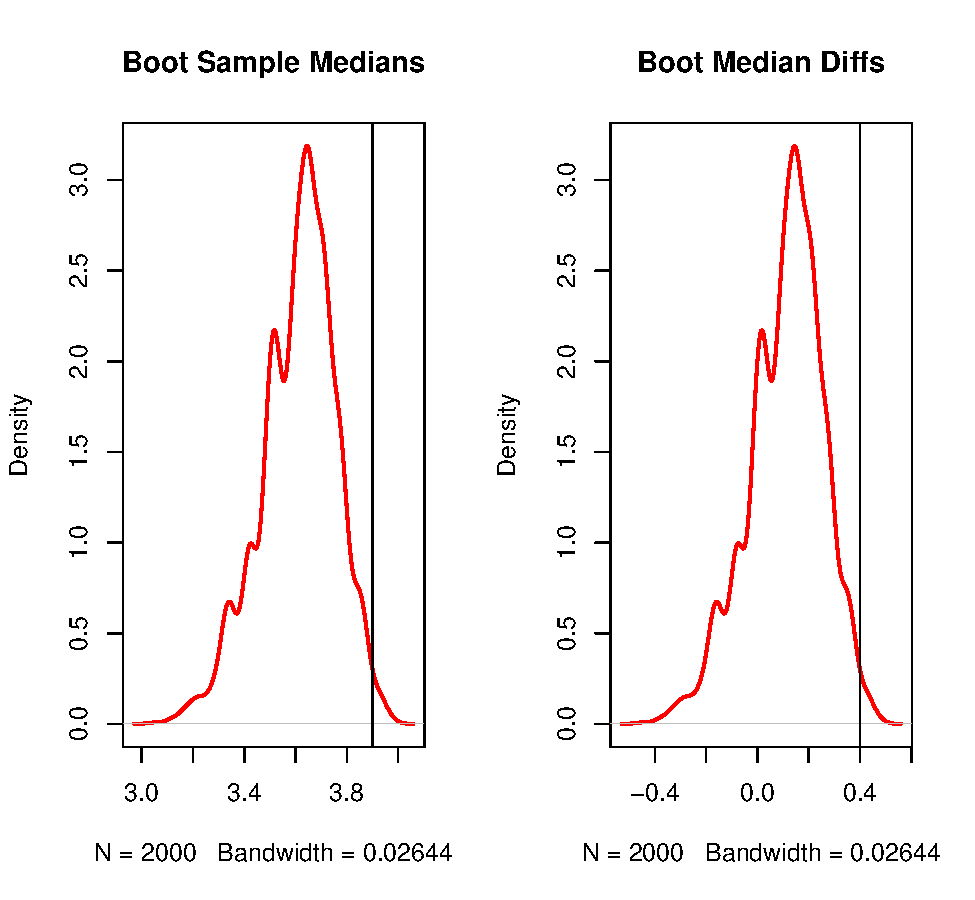
\includegraphics[width=0.9\linewidth]{bacs_hw4_files/figure-latex/unnamed-chunk-10-1}

\hypertarget{iv-what-is-your-conclusion-about-verizons-claim-about-the-median-and-why}{%
\paragraph{(iv) What is your conclusion about Verizon's claim about the
median, and
why?}\label{iv-what-is-your-conclusion-about-verizons-claim-about-the-median-and-why}}

We accept Null Hypothesis H0, since 3.5 clearly lies within the
estimated 99 \% CI.

\hypertarget{question-2}{%
\section{Question 2}\label{question-2}}

\begin{Shaded}
\begin{Highlighting}[]
\CommentTok{\# install.packages("remotes")}
\CommentTok{\# remotes::install\_github("soumyaray/compstatslib")}
\CommentTok{\# library(compstatslib)}
\CommentTok{\# compstatslib::interactive\_t\_test()}
\end{Highlighting}
\end{Shaded}

\hypertarget{instruction-3}{%
\subsection{Instruction}\label{instruction-3}}

Your colleague, a data analyst in your organization, is working on a
hypothesis test where he has sampled product usage information from
customers who are using a new smartwatch. He wishes to test whether the
mean usage time is higher than the usage time of the company's previous
smartwatch released two years ago:

\textbf{H\_null} : The mean usage time of the new smartwatch is the same
or less than for the previous smartwatch

\textbf{H\_alt} : The mean usage time is greater than that of our
previous smartwatch

After collecting data from just n=50 customers, he informs you that he
has found diff=0.3 and sd=2.9. Your colleague believes that we cannot
reject the null hypothesis at alpha of 5\%.

Consider the scenarios (a -- d) independently using the simulation tool.
For each scenario, start with the initial parameters above, then adjust
them to answer the following questions:

1. Would this scenario create systematic or random error (or both or
neither)?\\
2. Which part of the t-statistic or significance (diff, sd, n, alpha)
would be affected?\\
3. Will it increase or decrease our power to reject the null
hypothesis?\\
4. Which kind of error (Type I or Type II) becomes more likely because
of this scenario?

\hypertarget{a-1}{%
\subsection{2a}\label{a-1}}

\hypertarget{scenario}{%
\subsubsection{\texorpdfstring{\textbf{Scenario}}{Scenario}}\label{scenario}}

You discover that your colleague wanted to target the general population
of Taiwanese users of the product. However, he only collected data from
a pool of young consumers, and missed many older customers who you
suspect might use the product much less every day.

\hypertarget{answer}{%
\subsubsection{\texorpdfstring{\textbf{Answer}}{Answer}}\label{answer}}

\begin{enumerate}
\def\labelenumi{\arabic{enumi}.}
\tightlist
\item
  systemic error
\item
  If it is the case that older customers use the device less frequently
  than their younger counterparts, then the diff is likely to be
  greater.
\item
  increase
\item
  type I error rate (alpha)
\end{enumerate}

\hypertarget{b-1}{%
\subsection{2b}\label{b-1}}

\hypertarget{scenario-1}{%
\subsubsection{\texorpdfstring{\textbf{Scenario}}{Scenario}}\label{scenario-1}}

You find that 20 of the respondents are reporting data from the wrong
wearable device, and should not have been in the sample. These 20 people
are just like the others in every other respect.

\hypertarget{answer-1}{%
\subsubsection{\texorpdfstring{\textbf{Answer}}{Answer}}\label{answer-1}}

\begin{enumerate}
\def\labelenumi{\arabic{enumi}.}
\tightlist
\item
  random error
\item
  The unwanted responses from the sample is likely to inflate the sample
  size, and by se formula larger sample sizes contribute to greater
  standard error.
\item
  decrease
\item
  type II error rate (beta)
\end{enumerate}

\hypertarget{c-1}{%
\subsection{2c}\label{c-1}}

\hypertarget{scenario-2}{%
\subsubsection{\texorpdfstring{\textbf{Scenario}}{Scenario}}\label{scenario-2}}

A very annoying professor visiting your company has criticized your
colleague's ``95\% confidence'' criteria, and has suggested relaxing it
to just 90\%.

\hypertarget{answer-2}{%
\subsubsection{\texorpdfstring{\textbf{Answer}}{Answer}}\label{answer-2}}

\begin{enumerate}
\def\labelenumi{\arabic{enumi}.}
\tightlist
\item
  neither
\item
  The significance level (alpha) is relaxed from 0.05 to 0.10.
\item
  increase
\item
  type I error rate (alpha)
\end{enumerate}

\hypertarget{d}{%
\subsection{2d}\label{d}}

\hypertarget{scenario-3}{%
\subsubsection{\texorpdfstring{\textbf{Scenario}}{Scenario}}\label{scenario-3}}

Your colleague has measured usage times on five weekdays and taken a
daily average. But you feel this will underreport usage for younger
people who are very active on weekends, whereas it over-reports usage of
older users.

\hypertarget{answer-3}{%
\subsubsection{\texorpdfstring{\textbf{Answer}}{Answer}}\label{answer-3}}

\begin{enumerate}
\def\labelenumi{\arabic{enumi}.}
\tightlist
\item
  systemic error
\item
  If it is the case that older customers use the device less frequently
  than their younger counterparts, then the diff is likely to be
  smaller.
\item
  decrease
\item
  type II error rate (beta)
\end{enumerate}

\end{document}
